% cap2.tex

\chapter{Bibliographic Revision}
\label{ch:litRev} % la etiqueta para referencias

% {\color{blue} En esta sección de debe incluir la revisión general y especifica de la investigación
% desarrollada en la tesis.
% Aparte de referencias antiguas, las citas deben incluir referencias sustanciales de
% los 5 últimos años que den cuenta de la situación actual del tema a investigar,
% evitar el uso de páginas web o fuentes no formales de información. (Máximo 15 páginas). }
% $\lfloor x \rfloor$

\color{blue}{This section provides a comprehensive literature review of the key topics and concepts relevant to this research....}


\section{Section 1}



\begin{figure}[H]
\label{fig:RNN}
\centering
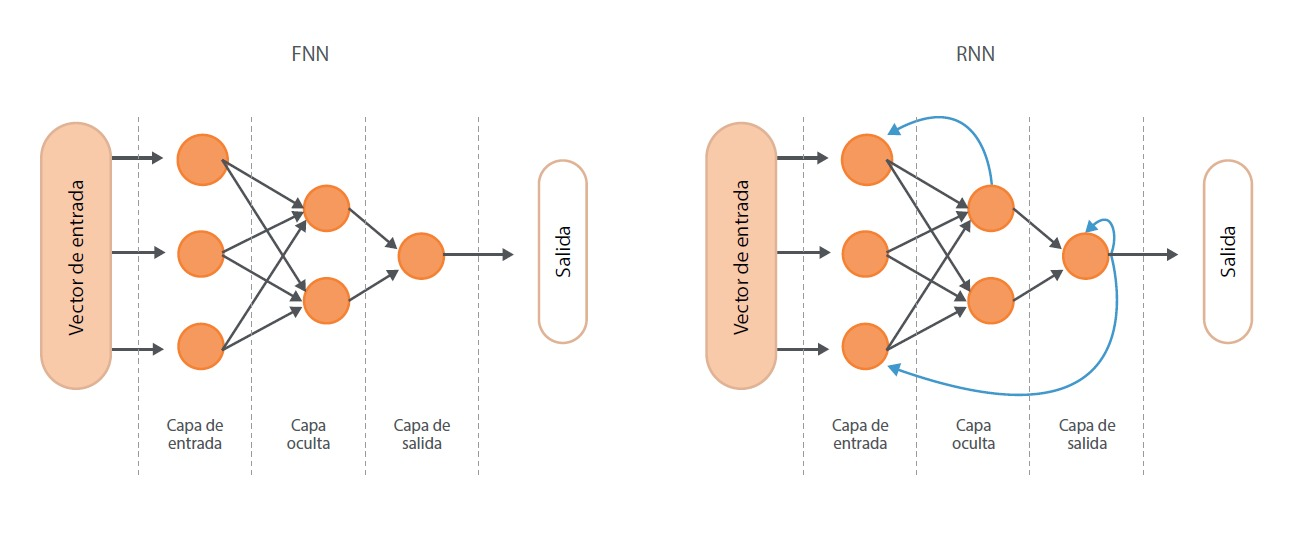
\includegraphics[scale=0.2]{images/RNNFNN.jpeg}
\caption[FNN, and RNN Architectures]{FNN, and RNN Architectures, Source: \cite{maldonado2022analytics}}
\end{figure}

Another significant advancement in NLP came with the introduction of Convolutional Neural Networks (CNNs).The convolution operation is defined as follows:
\[
(f * g)(x, y) = \sum_{i=0}^{m-1} \sum_{j=0}^{n-1} f(i, j) \cdot g(x-i, y-j)
\]
Where:
\begin{enumerate}
    \item $f$ and $g$ represent the input image and filter respectively.
    \item $m$ and $n$ denote the dimensions of the filter.
    \item $(x, y)$ are the spatial coordinates of the output feature map.
\end{enumerate}



The multi-head self-attention mechanism computes three important matrices: Query (Q), Key (K), and Value (V). These matrices are obtained from the input sequence. The self-attention mechanism calculates a weighted sum of the values (V) based on the compatibility scores (dot products) between the queries (Q) and keys (K). The intuition is that the model can focus on different parts of the input sequence (values) based on the importance of each word (queries and keys).

The self-attention operation can be formulated as follows, for a single attention head:

\[
\text{Attention}(Q, K, V) = \text{softmax}\left(\frac{QK^T}{\sqrt{d_k}}\right)V
\]

Where:
\begin{itemize}
    \item \(Q\), \(K\), and \(V\) are the query, key, and value matrices, respectively, derived from the input sequence.
    \item \(d_k\) is the dimension of the query and key vectors.
\end{itemize}
\vspace{0.5cm}

In the following subsections, we will delve into the details of pre-training and fine-tuning Transformers models, highlighting the methodologies and techniques involved, but first hyperparameters must be explained since they are relevant in both phases.

\subsection{HyperParameters}
Hyperparameters are configuration settings that determine the behavior and performance of a machine learning model \cite{Goodfellow-et-al-2016}. They are set before the training process and are not learned from the data. These parameters govern various aspects of the training process and can significantly impact the model's performance. Different models and tasks may require different hyperparameters to achieve optimal results \cite{bergstra2012random}. Some common hyperparameters include the learning rate, batch size, number of training epochs, weight decay, warm-up ratio, and max sequence length. Let's focus on two key hyperparameters: learning rate and batch size.

\begin{itemize}[]
\item The learning rate controls the step size at which the model's parameters are updated during training. A higher learning rate allows for faster convergence but may risk overshooting the optimal solution. On the other hand, a lower learning rate ensures more stable updates but might lead to slower convergence \cite{series/lncs/Bottou12}. Choosing an appropriate learning rate involves a trade-off between convergence speed and stability.
\item The batch size refers to the number of samples used in each iteration of the training process. Larger batch sizes tend to provide smoother and more stable updates due to the averaging effect across multiple samples. However, larger batch sizes require more memory and computational resources, which can be a constraint for larger models or limited hardware. In such cases, reducing the batch size becomes necessary to fit the model into memory and maintain efficient training \cite{keskar2017largebatch}.
\end{itemize}

